\documentclass{article}
\usepackage[utf8]{inputenc}
\usepackage[export]{adjustbox}
\usepackage{subfigure}
\usepackage{url}
\usepackage{graphicx}
\graphicspath {
	{images/}
}

\begin{document}

\title{Prototyping}
\author{Cardspark - Group 26}
\date{\today}
\maketitle

Used FluidUI to prototype our idea and get a feel for the design and whether the card format would be concise enough for revision notes.
\begin{figure}[ht]
	\centering
	\begin{subfigure}{}
	  \centering
			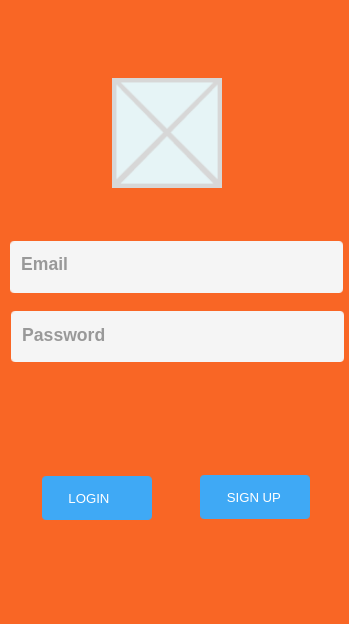
\includegraphics[scale=0.3]{fluidlogin.png}
	\end{subfigure}%
	\begin{subfigure}{}
	  \centering
			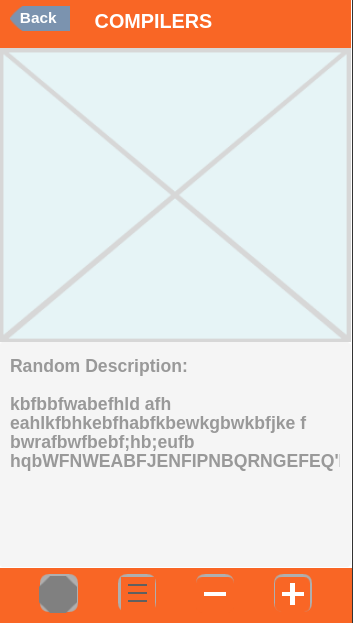
\includegraphics[scale=0.3]{fluidcard.png}
	\end{subfigure}
\end{figure}

(Placeholder)
\begin{center}
	\vspace{1mm}
	
\includegraphics[scale=0.2]{placeholder.png}
	\vspace{1mm}
\end{center}

\newpage

During the technical implementation of our application, we made use of our iOS phones to demo our app and allow ourselves and other users to test the app and look for improvements.

\begin{center}
	\vspace{1mm}
	
\includegraphics[scale=0.2]{placeholder.png}
	\vspace{1mm}
\end{center}

One such improvement was...
Another we made due to user feedback was...


\end{document}
